\documentclass[11pt, a4paper]{article}

\usepackage{seqsplit}
\usepackage{hyperref}
\usepackage{graphicx}



\begin{document}

De vierde ciphertekst was versleuteld met Enigma. Eerst implementeerden we een volledige Enigma machine. Daarna gingen we op zoek naar de gebruikte rotoren en hun beginstand. Er was een crib gegeven, dus we konden makkelijk een crib graph opstellen. Hiervoor stelden we manueel een .dot file om, waarmee we een visuele voorstelling genereerden. Deze is hieronder weegegeven. \\
\begin{center}
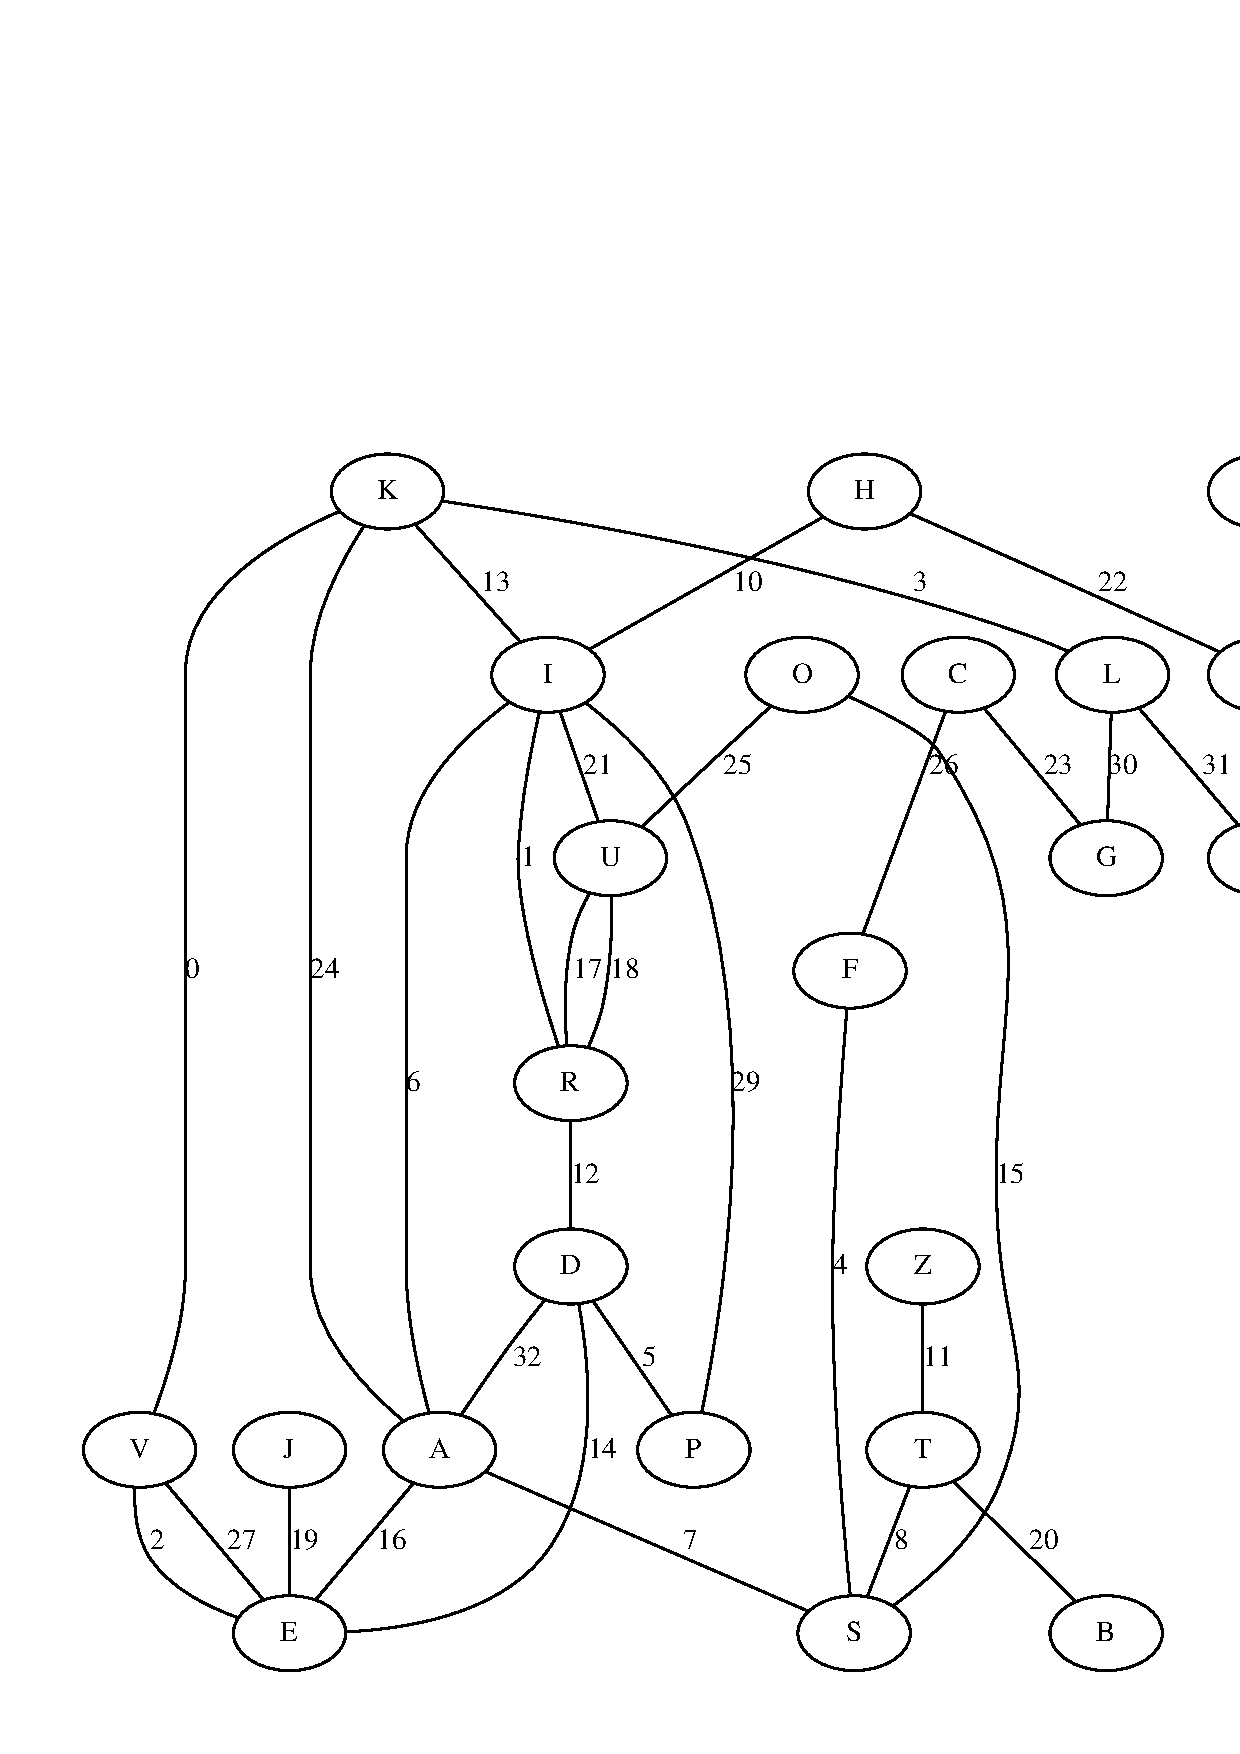
\includegraphics[scale=0.25]{graph.png}
\end{center}  
Aan de hand van de graph konden we op zoek naar gesloten paden. Door de lengte van de crib waren er heel wat mogelijkheden. We bepaalden voor de letter U 6 gesloten paden. We gingen dan, met elke mogelijke volgorde van rotoren, op zoek naar een k waarvoor een letter invariant bleef op elk van die paden. Hiervoor was een kleine modificatie aan onze ge\"implementeerde Engima machine voldoende. We vonden dat er hiervoor slechts \'e\'en optie was, namelijk rotorvolgorde 420 met als beginstand KSY. De invariante letter was hier de U, wat betekent dat de U door het plugboard niet aangepast wordt. We herhaalden deze test met de letters A, D en I, waarvoor we ook telkens 5 \`a 6 gesloten paden zochten. Hier vonden we ook telkens slechts 1 of 2 resultaten, waaronder altijd rotorvolgorde 420 met beginstand KSY. Dit was dus zeker het juiste antwoord. Uit deze resultaten vonden we ook dat het plugboard I en Y verwisselt, en de A en de D niet aanpast. Nu moesten we enkel nog op zoek naar de rest van het plugboard. Omdat we een behoorlijk grote crib hadden, waren er voor de meeste letters gesloten paden te vinden in de graph. We konden dus gewoon een versimpelde versie van de voorgaande code draaien voor elke letter met gesloten paden om het plugboard verder te bepalen. Hiervoor hoefden we de test enkel voor de correcte rotorvolgorde en beginstand draaien. De enige letters zonder gesloten paden waren B, J, Q, T, W, X, Y en Z waarbij Q, W en X helemaal niet in de graph voorkwamen, en we al wisten dat Y met I werd omgewisseld. We gingen dus enkel de mappings van de letters met gesloten paden zoeken. Hierdoor vonden we ook de mappings voor B, Q, W en Z omdat ze elk verwisseld werden met een letter die wel gesloten paden had. We hadden het plugboard dus op J, T en X na bepaald. Er waren nu echter maar 4 mogelijke plugboards over: ofwel werden twee van de drie letters met elkaar gewisseld ofwel werd geen enkele gewisseld. Door de ciphertekst met elk van de vier opties te decipheren, vonden we dat enkel die waarbij J, T en X niet werden aangepast de crib juist ontcijferde en dus juist was. Hiermee hadden we ook het plugboard volledig bepaald en konden we de tekst volledig ontcijferen. Het was een deel uit Die Blechtrommel van G\"unter Grass \footnote{\url{http://www.lawrenceglatz.com/germ3230/texte/grass1.htm}}.



Rotorvolgorde: 420 \\
Beginstand: KSY \\
Plugboard:  KEDCHGFYJBLWNZPSRQTUVMXIO \\
Verwisselingen in plugboard: B-K, C-E, F-H, I-Y, M-W, O-Z, Q-S \\
\seqsplit{VIELSPASSMITDIESERUEBUNGAUFENIGMAZUGEGEBENICHBININSASSEEINERHEILUNDPFLEGEANSTALTMEINPFLEGERBEOBACHTETMICHLASSTMICHKAUMAUSDEMAUGEDENNINDERTURISTEINGUCKLOCHUNDMEINESPFLEGERSAUGEISTVONJENEMBRAUNWELCHESMICHDENBLAUAUGIGENNICHTDURCHSCHAUENKANNMEINPFLEGERKANNALSOGARNICHTMEINFEINDSEINLIEBGEWONNENHABEICHIHNERZAHLEDEMGUCKERHINTERDERTURSOBALDERMEINZIMMERBETRITTBEGEBENHEITENAUSMEINEMLEBENDAMITERMICHTROTZDESIHNHINDERNDENGUCKLOCHESKENNENLERNTDERGUTESCHEINTMEINEERZAHLUNGENZUSCHATZENDENNSOBALDICHIHMETWASVORGELOGENHABEZEIGTERMIRUMSICHERKENNTLICHZUGEBENSEINNEUESTESKNOTENGEBILDEOBEREINKUNSTLERISTBLEIBEDAHINGESTELLTEINEAUSSTELLUNGSEINERKREATIONENWURDEJEDOCHVONDERPRESSEGUTAUFGENOMMENWERDENAUCHEINIGEKAUFERHERBEILOCKENERKNOTETORDINAREBINDFADENDIEERNACHDENBESUCHSSTUNDENINDENZIMMERNSEINERPATIENTENSAMMELTUNDENTWIRRTZUVIELSCHICHTIGVERKNORPELTENGESPENSTERNTAUCHTDIESEDANNINGIPSLASSTSIEERSTARRENUNDSPIESSTSIEMITSTRICKNADELNDIEAUFHOLZSOCKELCHENBEFESTIGTSINDOFTSPIELTERMITDEMGEDANKENSEINEWERKEFARBIGZUGESTALTENICHRATEDAVONABWEISEAUFMEINWEISSLACKIERTESMETALLBETTHINUNDBITTEIHNSICHDIESESVOLLKOMMENSTEBETTBUNTBEMALTVORZUSTELLENENTSETZTSCHLAGTERDANNSEINEPFLEGERHANDEUBERDEMKOPFZUSAMMENVERSUCHTINETWASZUSTARREMGESICHTALLENSCHRECKENGLEICHZEITIGAUSDRUCKZUGEBENUNDNIMMTABSTANDVONSEINENFARBIGENPLANENMEINWEISSLACKIERTESMETALLENESANSTALTSBETTISTALSOEINMASSSTABMIRISTESSOGARMEHRMEINBETTISTDASENDLICHERREICHTEZIELMEINTROSTISTESUNDKONNTEMEINGLAUBEWERDENWENNMIRDIEANSTALTSLEITUNGERLAUBTEEINIGEANDERUNGENVORZUNEHMENDASBETTGITTERMOCHTEICHERHOHENLASSENDAMITMIRNIEMANDMEHRZUNAHETRITTEINMALINDERWOCHEUNTERBRICHTEINBESUCHSTAGMEINEZWISCHENWEISSENMETALLSTABENGEFLOCHTENESTILLEDANNKOMMENSIEDIEMICHRETTENWOLLENDENENESSPASSMACHTMICHZULIEBENDIESICHINMIRSCHATZENACHTENUNDKENNENLERNENMOCHTENWIEBLINDNERVOSWIEUNERZOGENSIESINDKRATZENMITIHRENFINGERNAGELSCHERENANMEINEMWEISSLACKIERTENBETTGITTERKRITZELNMITIHRENKUGELSCHREIBERNUNDBLAUSTIFTENDEMLADELANGGEZOGENEUNANSTANDIGESTRICHMANNCHENMEINANWALTSTULPTJEDESMALSOBALDERMITSEINEMHALLODASZIMMERSPRENGTDENNYLONHUTUBERDENLINKENPFOSTENAMFUSSENDEMEINESBETTESSOLANGESEINBESUCHWAHRTUNDANWALTEWISSENVIELZUERZAHLENRAUBTERMIRDURCHDIESENGEWALTAKTDASGLEICHGEWICHTUNDDIEHEITERKEITNACHDEMMEINEBESUCHERIHREGESCHENKEAUFDEMWEISSENMITWACHSTUCHBEZOGENENTISCHCHENUNTERDEMANEMONENAQUARELLDEPONIERTHABENNACHDEMESIHNENGELUNGENISTMIRIHREGERADELAUFENDENODERGEPLANTENRETTUNGSVERSUCHEZUUNTERBREITENUNDMICHDENSIEUNERMUDLICHRETTENWOLLENVOMHOHENSTANDARDIHRERNACHSTENLIEBEZUUBERZEUGENFINDENSIEWIEDERSPASSANDEREIGENENEXISTENZUNDVERLASSENMICHDANNKOMMTMEINPFLEGERUMZULUFTENUNDDIEBINDFADENDERGESCHENKPACKUNGENEINZUSAMMELNOFTMALSFINDETERNACHDEMLUFTENNOCHZEITANMEINEMBETTSITZENDBINDFADENAUFDROSELNDSOLANGESTILLEZUVERBREITENBISICHDIESTILLEBRUNOUNDBRUNODIESTILLENENNEBRUNOMUNSTERBERGICHMEINEJETZTMEINENPFLEGERLASSEDASWORTSPIELHINTERMIRKAUFTEAUFMEINERECHNUNGFUNFHUNDERTBLATTSCHREIBPAPIERBRUNODERUNVERHEIRATETKINDERLOSISTUNDAUSDEMSAUERLANDSTAMMTWIRDSOLLTEDERVORRATNICHTREICHENDIEKLEINESCHREIBWARENHANDLUNGINDERAUCHKINDERSPIELZEUGVERKAUFTWIRDNOCHEINMALAUFSUCHENUNDMIRDENNOTWENDIGENUNLINIERTENPLATZFURMEINHOFFENTLICHGENAUESERINNERUNGSVERMOGENBESCHAFFENNIEMALSHATTEICHMEINEBESUCHERETWADENANWALTODERKLEPPUMDIESENDIENSTBITTENKONNENBESORGTEMIRVERORDNETELIEBEHATTEDENFREUNDENSICHERVERBOTENETWASSOGEFAHRLICHESWIEUNBESCHRIEBENESPAPIERMITZUBRINGENUNDMEINEMUNABLASSIGSILBENAUSSCHEIDENDENGEISTZUMGEBRAUCHFREIZUGEBENALSICHZUBRUNOSAGTEACHBRUNOWURDESTDUMIRFUNFHUNDERTBLATTUNSCHULDIGESPAPIERKAUFENANTWORTETEBRUNOZURZIMMERDECKEBLICKENDUNDSEINENZEIGEFINGEREINENVERGLEICHHERAUSFORDERNDINDIEGLEICHERICHTUNGSCHICKENDSIEMEINENWEISSESPAPIERHERROSKAR}

\end{document}
